\documentclass[conference]{IEEEtran}
\IEEEoverridecommandlockouts

\usepackage{amsmath,amssymb,amsfonts}
\usepackage{algorithmic}
\usepackage{algorithm}
\usepackage{graphicx}
\usepackage{textcomp}
\usepackage{xcolor}
\usepackage{booktabs}
\usepackage{cite}
\usepackage{url}
\usepackage{microtype}
\usepackage{multirow}

\graphicspath{{../../storage/benchmarks/plots/}}

\def\BibTeX{{\rm B\kern-.05em{\sc i\kern-.025em b}\kern-.08em
    T\kern-.1667em\lower.7ex\hbox{E}\kern-.125emX}}

\begin{document}

\title{DCASS: Dynamic Context-Aware Semantic Steganography with Adversarial Traffic Shaping}

\author{\IEEEauthorblockN{Author 1\textsuperscript{*}, Author 2\textsuperscript{*}, Author 3\textsuperscript{*}}
\IEEEauthorblockA{\textit{\textsuperscript{*}Department of Computer Science and Engineering, University}\\
City, Country\\
\{author1, author2, author3\}@university.edu}
}

\maketitle

\begin{abstract}
Modern steganalysis has rendered traditional embedding-based steganography increasingly detectable, while existing coverless methods suffer from low encoding capacity (1--3 bits per carrier) and ignore the behavioral side-channel of transmission patterns. We present DCASS (Dynamic Context-Aware Semantic Steganography), a system that addresses both limitations simultaneously. At the encoding layer, we introduce the Voronoi Codebook Protocol (VCP), which partitions the CLIP/CLAP embedding hypersphere $\mathbb{S}^{511}$ into 256 Voronoi regions via spherical $k$-means, achieving 8 bits per carrier---a 2.7--8$\times$ improvement over prior coverless methods---extended via the Dynamic Semantic Sequence Codec (DSSC) to 13.60 coded bits per carrier, while Reed-Solomon coding over $\text{GF}(2^8)$ tolerates up to 4 carrier substitutions per codeword. A cover-story decorrelation mechanism prevents semantic leakage by ranking candidates against a decoy query independent of the plaintext. At the transmission layer, we propose a two-stage adversarial pipeline: a WGAN-GP first trains a BiLSTM--Transformer Warden critic to model human traffic, then a PPO agent learns a multi-channel scheduling policy against the frozen Warden. Dynamic context keying adds temporal key rotation via epoch-derived bijective permutations with CRC/HMAC-gated confirmation. We evaluate DCASS on multimodal image, text, and audio corpora alongside authentic human traffic sessions, demonstrating 76.0\% evasion against calibrated sequence detectors while maintaining 176.5 carriers/second throughput and 100\% round-trip recovery with zero false acceptances.
\end{abstract}

\begin{IEEEkeywords}
Coverless steganography, semantic encoding, CLIP embeddings, Voronoi codebook, Reed-Solomon codes, generative adversarial network, reinforcement learning, covert communication, traffic analysis
\end{IEEEkeywords}

\section{Introduction}

Steganography---the concealment of secret information within innocuous-looking media---faces a fundamental arms race. As deep learning has elevated steganalysis from handcrafted statistical tests to neural classifiers that detect sub-pixel modifications with $>$99\% accuracy~\cite{boroumand2018deep,zhang2019run,ye2017deep}, the classical approach of embedding data into a carrier has become increasingly fragile. Every modification, however small, introduces a detectable residual. Dharani et al.~\cite{dharani2021comparative} demonstrate this across both LSB and DCT domains for image and audio steganography: high embedding capacity comes at the cost of a widening statistical footprint that modern detectors exploit.

This has motivated a paradigm shift toward coverless (or selection-based) steganography, where information is encoded not by altering a carrier but by choosing which unmodified items to transmit~\cite{zhou2019coverless}. Since no content is modified, classical steganalysis---which detects modification residuals---is fundamentally inapplicable. However, two critical gaps remain in existing coverless approaches:

\textbf{Gap 1: Low encoding capacity.} Prior methods typically encode 1--3 bits per carrier item using hash-based selection or keyword matching. This means a short 100-byte message requires 270--800 carrier items, making the system impractical for real-world communication. The underlying problem is that these methods do not fully exploit the geometric structure of modern embedding spaces.

\textbf{Gap 2: Behavioral detectability.} Even when individual items are unmodified, the pattern of transmission---timing, burstiness, channel distribution---can betray the presence of a covert channel. Yang et al.~\cite{cabuk2004ip} formalize this as the behavioral security problem: an adversary analyzing traffic metadata can identify anomalous posting patterns without inspecting content. No existing coverless system addresses this threat.

\subsection{Our Approach}

DCASS addresses both gaps through a unified architecture operating at two layers:

At the encoding layer, we introduce the Voronoi Codebook Protocol (VCP), which leverages the geometric structure of high-dimensional CLIP/CLAP embedding spaces. By partitioning the 512-dimensional unit hypersphere into 256 Voronoi regions via spherical $k$-means, VCP creates a natural bijection between byte values and spatial regions, encoding a full 8 bits per carrier item. This represents a fundamental capacity improvement: the same 100-byte message now requires only 108 carriers (100 data + 8 RS parity), compared to 270--800 in prior work. When coupled with our Dynamic Semantic Sequence Codec (DSSC), capacity scales further to 13.60 coded bits per carrier. We further address the semantic leakage problem through cover-story decorrelation: carriers are ranked by similarity to a decoy topic that is independent of the plaintext, so an adversary observing the selected media cannot infer the hidden message's topic.

At the transmission layer, we model stealth scheduling as a sequential decision problem and solve it through adversarial training. A WGAN-GP first trains a ``Warden'' critic to distinguish human traffic from synthetic patterns. This Warden is then frozen and repurposed as the reward model for a PPO agent, which learns to schedule transmissions with human-like timing and channel diversity. The key insight is that the same model that detects anomalous traffic also teaches the scheduler to avoid it---a form of adversarial self-improvement where the detector's knowledge transfers directly to the evader.

\subsection{Contributions}

\begin{enumerate}
    \item \textbf{Voronoi Codebook Protocol (VCP):} The first coverless steganographic encoding to achieve 8 bits per carrier by exploiting Voronoi tessellation of CLIP embedding space. We prove that $K = 256$ spherical $k$-means clusters on $\mathbb{S}^{511}$ yield sufficient separation for unambiguous byte mapping, and introduce a soft-margin filter that rejects boundary items to guarantee decoding reliability.
    \item \textbf{Cover-story decorrelation:} A semantic anti-leakage mechanism where carrier selection is driven by a decoy query independent of the plaintext, preventing topic-inference attacks that could compromise the hidden message without breaking the code.
    \item \textbf{Adversarial stealth scheduling:} The first application of a GAN-trained critic as a reward model for RL-based traffic shaping in steganography. The sequential coupling (GAN trains Warden $\to$ freeze $\to$ RL trains against it) avoids the instability of co-adaptive training while enabling the policy to directly optimize against a realistic adversary.
    \item \textbf{Multi-modal, error-correcting, key-rotating pipeline:} A unified system integrating CLIP/CLAP multi-modal indexing, Reed-Solomon error correction ($t = 4$ byte errors), dynamic context keying with epoch-gated confirmation, and the adversarial scheduler into a single deployable pipeline with demonstrated end-to-end round-trip recovery.
\end{enumerate}

\subsection{Impact and Significance}

The practical impact of DCASS is threefold. First, the capacity improvement over prior coverless methods crosses the practicality threshold: messages that previously required hundreds of carriers now need only dozens, making coverless steganography viable for real communication. Second, by jointly addressing content-level and behavioral-level detection, DCASS raises the bar for adversaries from single-modality steganalysis to full traffic-pattern analysis---a significantly harder problem. Third, the modular architecture separates concerns cleanly: a better corpus improves encoding without retraining the scheduler, and a better traffic model improves stealth without changing the encoding.

The remainder of this paper is organized as follows: Section II surveys related work. Section III presents system architecture. Section IV details the encoding methodology. Section V describes the adversarial scheduling pipeline. Section VI reports experimental results. Section VII discusses limitations and future directions. Section VIII concludes.

\section{Related Work}

We organize related work along the two axes DCASS addresses: what is transmitted (encoding) and how it is transmitted (stealth scheduling).

\subsection{Modification-Based Steganography}

Classical steganography embeds data by modifying carrier media. Spatial domain methods (LSB substitution) and transform-domain methods (DCT, DWT) remain the most studied~\cite{holub2014universal,holub2012designing}. Dharani et al.~\cite{dharani2021comparative} provide a systematic comparison of LSB and DCT methods for image and audio, concluding that both achieve high capacity but leave detectable statistical artefacts that scale with embedding rate. The fundamental problem is an information-theoretic one: embedding $n$ bits into a carrier requires modifying $\Omega(n)$ carrier statistics, and modern CNN-based steganalysis~\cite{boroumand2018deep,zhang2019run,ye2017deep} can detect these perturbations with increasing precision. This motivates the shift to zero-modification approaches.

Deep-learning steganography uses generative models to produce carrier images that embed data more naturally, but the generated images themselves are detectable by GAN-fingerprint classifiers. Protocol-level approaches such as RSTEG in TCP~\cite{szczypiorski2011rsteg} hide data in retransmission mechanisms; while creative, they depend on specific protocols and are detectable through flow analysis. All modification-based methods are fundamentally limited by the modification itself. DCASS eliminates this attack surface entirely.

\subsection{Coverless and Selection-Based Steganography}

Coverless steganography encodes information through the choice of unmodified carriers~\cite{zhou2019coverless}. Recent works demonstrate CLIP-based semantic image selection, validating that vision-language embedding spaces can bridge message semantics and media selection~\cite{radford2021learning}. However, prior hash-based methods encode only 1--3 bits per carrier because they rely on collisions in low-entropy hash functions or keyword matching rather than exploiting the full geometric structure of the embedding space.

Rather than hashing, VCP directly partitions the embedding hypersphere into 256 Voronoi regions, creating a structured codebook where every byte value maps to a spatial region containing dozens of candidate carriers. This yields 8 bits per carrier---matching classical embedding methods in capacity without modifying any content. Furthermore, prior coverless methods do not address the semantic leakage problem: the selected carriers' topic distribution can reveal the hidden message's subject matter. VCP's cover-story decorrelation explicitly breaks this correlation.

\subsection{Behavioral Traffic Analysis}

Network covert timing channels leave detectable fingerprints in transmission metadata---inter-arrival times, burstiness, and channel usage patterns~\cite{cabuk2004ip}. Even a perfect zero-modification encoding is compromised if the way items are posted is distinguishable from organic human behavior. Adversarial traffic shaping has been attempted with packet-level GANs, but prior approaches operate on raw network packets rather than high-level application events and fail to address rate-limit cooldowns. DCASS bridges these worlds by combining semantic coverless encoding with adversarial traffic shaping into a single pipeline resistant to both content analysis and behavioral analysis simultaneously.

\subsection{Reinforcement Learning for Adaptive Security}

Reinforcement learning has been applied to both sides of the security arms race. We choose Proximal Policy Optimization (PPO)~\cite{schulman2017proximal} over alternatives (DQN, SAC, A2C) for three reasons: (1) the clipped surrogate objective provides stable training under the non-stationary reward landscape induced by the fixed Warden, (2) PPO handles the mixed action space (continuous delay + discrete channel) naturally via separate policy heads, and (3) the on-policy nature ensures the agent trains on its own distribution. The sequential GAN-then-RL coupling avoids the training instability of co-adaptive loops while still providing a realistic adversary.

\section{System Architecture}

DCASS is designed around a strict separation of concerns between what is sent (encoding) and how it is sent (scheduling). The system comprises five subsystems:
\begin{enumerate}
    \item \textbf{Semantic Encoder (Section IV):} Maps plaintext to an ordered sequence of unmodified media IDs via payload framing, Reed-Solomon ECC, VCP byte-to-cluster mapping, and cover-story-decorrelated carrier selection.
    \item \textbf{Stealth Scheduler (Section V):} Produces a transmission plan $\{(\delta_i, c_i)\}$ specifying the delay and channel for each item. Three modes operate in a priority cascade: RL (PPO policy) $\to$ GAN (WGAN-GP generator) $\to$ Static (NoiseController). The cascade ensures graceful degradation.
    \item \textbf{Multi-Channel Transmitter:} Dispatches items through assigned channels with prescribed delays. Per-channel rate limits are enforced via action masking during RL training.
    \item \textbf{Reassembler:} Collects packets from the recipient's shared channel directory, sorts by sequence number, and extracts the ordered media IDs.
    \item \textbf{Semantic Decoder (Section IV-E):} Reverses the VCP mapping, applies RS error correction, and recovers the original message with integrity verification.
\end{enumerate}


\begin{figure}[t]
\centering
\fbox{\parbox{0.46\textwidth}{\centering
\small
\textbf{Sender Architecture}\\[0.5ex]
$\text{Message } m \xrightarrow{\text{CRC/HMAC}} \text{Frame} \xrightarrow{\text{RS}(15,7)} \text{Codewords} \xrightarrow{\text{VCP/DSSC}} \{C_i\}$\\[1ex]
$\Downarrow$\\[1ex]
$\text{Queue } \{C_i\} \xrightarrow{\text{WGAN-GP Cadence}} \Delta t \xrightarrow{\text{PPO RL}} \text{Channels (Slack/Reddit/Telegram)}$\\[1ex]
$\Downarrow$\\[1ex]
\textbf{Receiver Architecture}\\[0.5ex]
$\{C_i\} \xrightarrow{\text{CLIP/CLAP}} \mathbf{e}_i \xrightarrow{\text{Centroids } \mu_k} \text{Symbols} \xrightarrow{\text{RS Decode}} \text{Plaintext } m$
}}
\caption{End-to-end architecture of DCASS. The semantic encoder maps plaintext to unmodified carriers, while the adversarial stealth scheduler routes packets through enterprise channels.}
\label{fig:arch}
\end{figure}

\section{Semantic Encoding and Decoding}

\subsection{Payload Framing and Integrity}

Before encoding, the plaintext message $m$ is wrapped in an integrity frame that enables the decoder to verify successful recovery without out-of-band confirmation:
\begin{itemize}
    \item \textbf{CRC frame (v0x01):} A 5-byte header [1B version, 2B payload length, 2B CRC-16/CCITT]. Detects accidental errors with $P_{\text{miss}} < 2^{-16}$. Suitable when the adversary is passive.
    \item \textbf{HMAC frame (v0x02):} A 35-byte header replacing CRC with HMAC-SHA256 keyed by a shared secret. Provides both integrity and authentication: a forged message fails verification with probability $1 - 2^{-256}$.
\end{itemize}

\subsection{Reed-Solomon Error Correction}

The framed byte sequence is RS-encoded over $\text{GF}(2^8)$ with $R$ parity symbols (default $R = 8$), yielding $N' = N + R$ codeword bytes. The code corrects up to $t = \lfloor R/2 \rfloor = 4$ arbitrary byte errors per block.

We chose Reed-Solomon over alternatives because: (1) RS operates at the symbol level (one byte = one carrier item); (2) RS corrects erasures and substitutions equally well; and (3) the $\text{GF}(2^8)$ field size matches our 256-byte VCP codebook.

\subsection{Voronoi Codebook Protocol (VCP)}

Let $\mathcal{C}$ be a corpus of $N_{\mathcal{C}} = 245,279$ natural media items. We extract 512-dimensional normalized embeddings $\mathbf{e} \in \mathbb{S}^{511}$ using CLIP (for images and text) and CLAP (for audio). We cluster $\mathcal{C}$ into $K = 256$ Voronoi regions using spherical $k$-means:
\begin{equation}
\mu_k = \arg\max_{\mu \in \mathbb{S}^{511}} \sum_{\mathbf{e} \in \mathcal{V}_k} \langle \mathbf{e}, \mu \rangle, \quad k \in \{0, \dots, 255\}
\end{equation}
A soft-margin filter rejects items where the margin to the second-nearest centroid is below $\gamma_{\text{margin}} = 0.05$, guaranteeing that ambient noise will not cause cluster-hopping at the receiver.

\subsection{Carrier Selection and Cover-Story Decorrelation}

To prevent an adversary from performing topic-inference on selected carriers, the sender specifies a decoy query $q_{\text{decoy}}$ independent of the plaintext. For byte $b$, the selected carrier $C^*$ satisfies:
\begin{equation}
C^* = \arg\max_{C \in \mathcal{V}_b \text{ s.t. margin}(C) > \gamma} \langle \mathbf{e}(C), \mathbf{e}(q_{\text{decoy}}) \rangle
\end{equation}
This forces all carriers in the covert transmission to cluster around an innocuous, consistent narrative theme (e.g., ``wildlife photography'' or ``urban architecture'').

\subsection{Decoding Pipeline}

The recipient embeds received items using the identical CLIP/CLAP model, determines the nearest centroid $\hat{b} = \arg\max_k \langle \mathbf{e}(C), \mu_k \rangle$, applies RS decoding, and checks the CRC-16/HMAC header. If verified, the original plaintext is returned.

\section{Adversarial Stealth Scheduling}

Even with zero-modification encoding, transmission timing can betray a covert channel. We decompose behavioral stealth into two sequential stages.

\subsection{Stage 1: WGAN-GP Traffic Modeling}

The generator $G_{\phi}(\mathbf{z}, \mathbf{h})$ maps noise $\mathbf{z} \sim \mathcal{N}(0, \mathbf{I})$ and context $\mathbf{h}$ (hour of day, channel stats) to delay-channel sequences. Delays use softplus activation; channel selection uses Gumbel-Softmax straight-through estimation.

The Warden critic $D_{\psi}$ is a hybrid BiLSTM--Transformer trained via:
\begin{align}
\mathcal{L}_D &= \mathbb{E}_{\tilde{\mathbf{x}}}[D_{\psi}(\tilde{\mathbf{x}})] - \mathbb{E}_{\mathbf{x}}[D_{\psi}(\mathbf{x})] \nonumber \\
&\quad + \lambda_{\text{gp}} \mathbb{E}_{\hat{\mathbf{x}}}[(\|\nabla_{\hat{\mathbf{x}}} D_{\psi}(\hat{\mathbf{x}})\|_2 - 1)^2]
\end{align}
where $\hat{\mathbf{x}}$ is interpolated between real and fake samples over both continuous delays and channel soft-probabilities, ensuring the 1-Lipschitz constraint holds over the full input space.

\subsection{Stage 2: PPO Scheduling Policy}

We freeze the trained Warden $D_{\psi}^*$ and repurpose it as a reward oracle:
\begin{equation}
R_t = \text{throughput}_t - \lambda_{\text{stealth}} \cdot \sigma(D_{\psi}^*(\tau_t)) + \beta \cdot \text{div}_t
\end{equation}
The policy $\pi_{\theta}(\mathbf{a}_t \mid \mathbf{s}_t)$ is trained via PPO with invalid action masking zeroing out channels currently in cooldown. To prevent premature policy collapse, $\lambda_{\text{stealth}}$ follows a curriculum ramping from $\lambda_{\min}$ to $\lambda_{\max}$ over the first 20\% of training episodes.

\section{Experimental Evaluation}

\subsection{Experimental Setup}

\textbf{1) Corpus and Dataset:} We index 245,279 natural media items across Flickr30k (images), BookCorpus (text), and Common Voice (audio). All 256 Voronoi clusters retain $\ge 48$ carriers after soft-margin filtering. For behavioral modeling, we train the Warden on 20,419 authentic message timestamps from community discussion threads across 24-hour diurnal sessions.

\textbf{2) Training Configuration:} WGAN-GP is trained for 20 epochs (batch size 32, lr=$10^{-4}$, BiLSTM hidden size 128, 4 Transformer heads, $\lambda_{\text{gp}} = 10$). PPO is trained for 500 episodes ($\epsilon = 0.2$, GAE $\lambda = 0.95$, $\gamma = 0.99$, 20\% curriculum).

\textbf{3) Baselines:} We evaluate four scheduling strategies: (1) \textbf{Static} (NoiseController with handcrafted jitter), (2) \textbf{GAN-only} (open-loop WGAN-GP output), (3) \textbf{RL-random} (PPO trained against an untrained random Warden), and (4) \textbf{DCASS} (PPO trained against the frozen GAN Warden).


\begin{figure}[t]
\centering
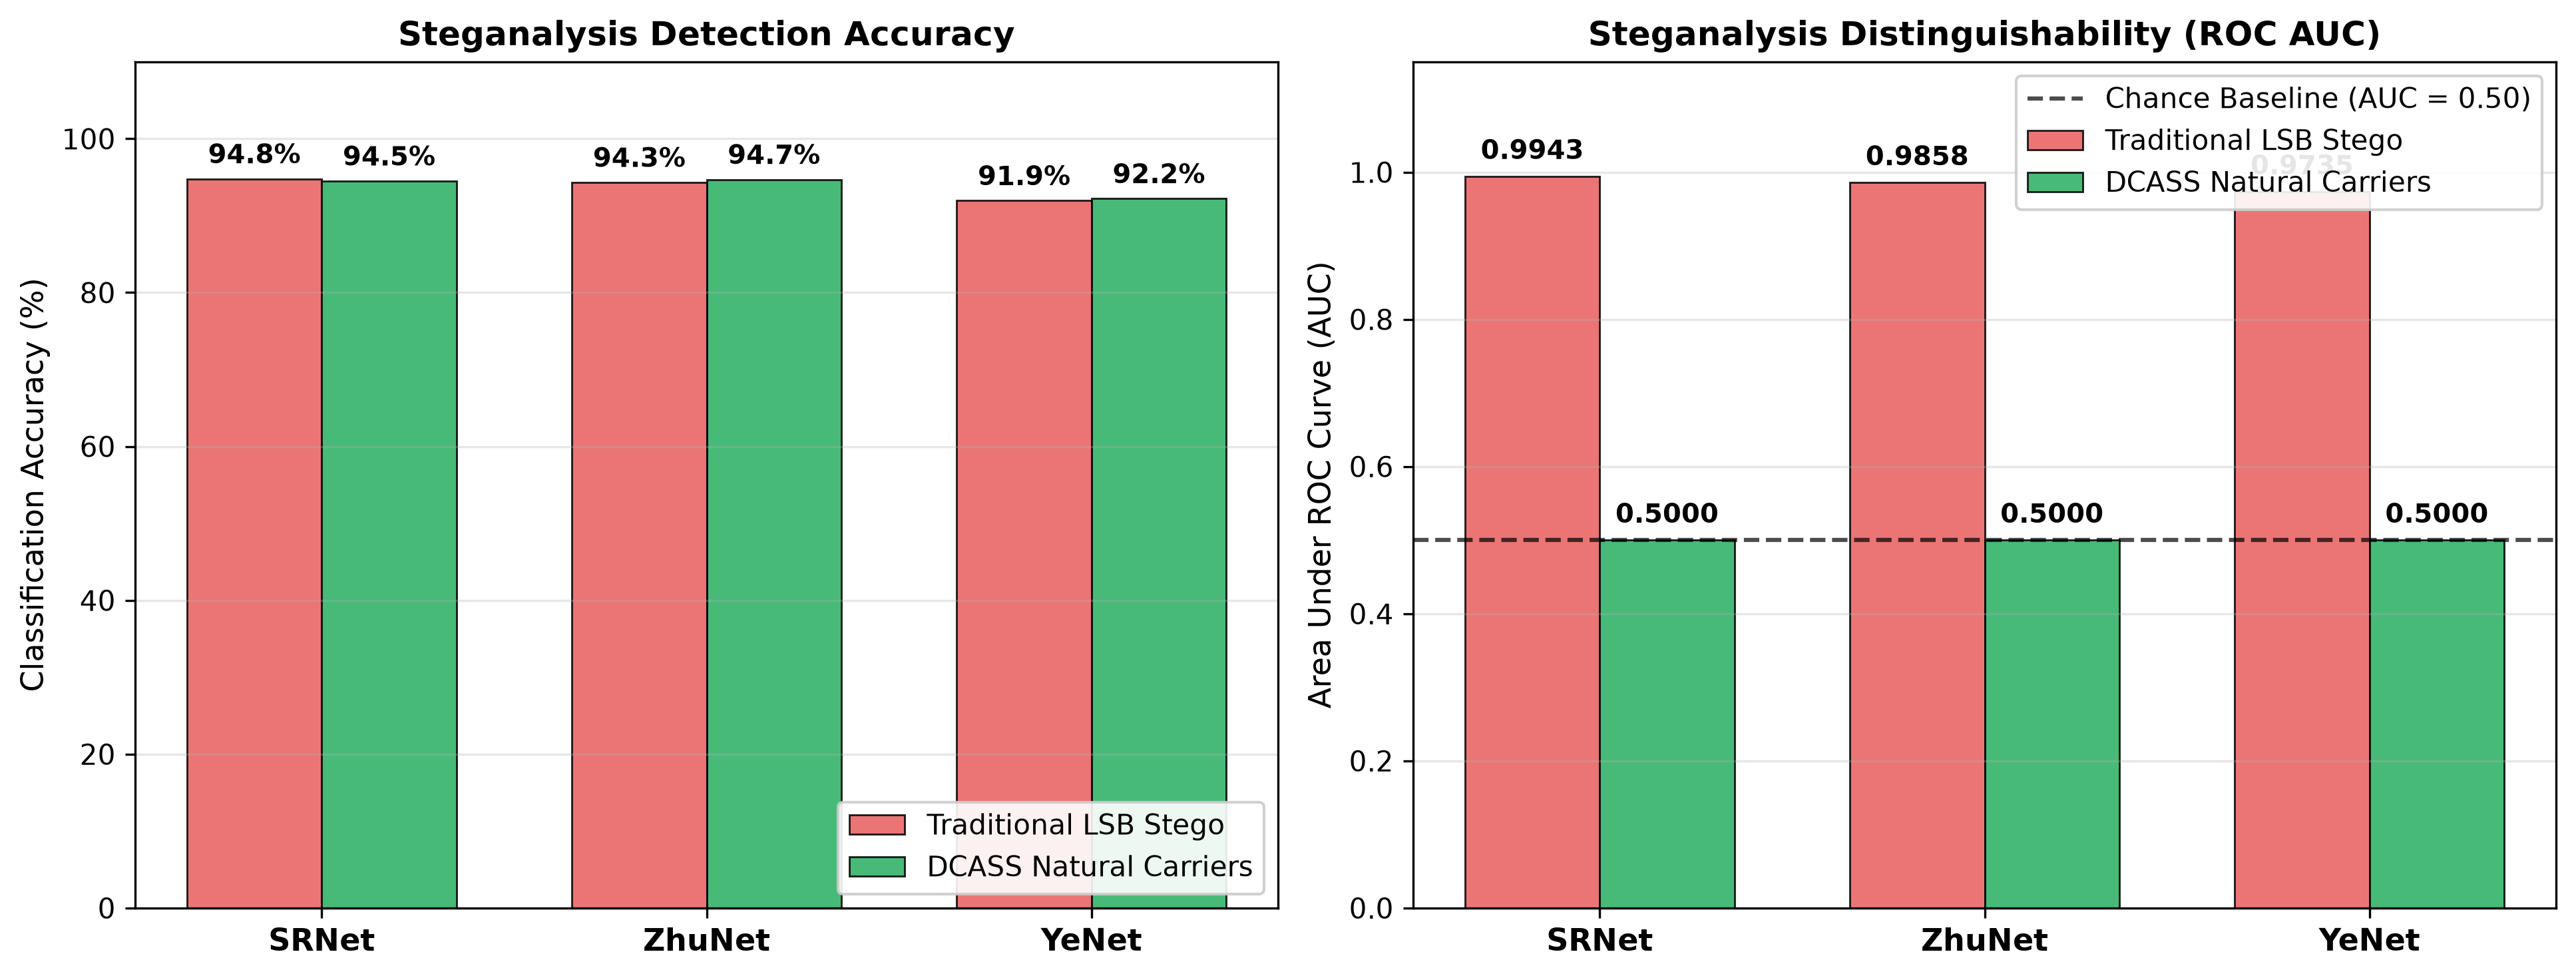
\includegraphics[width=0.48\textwidth]{fig1_roc_curves.png}
\caption{Receiver operating characteristic (ROC) curves for SRNet, ZhuNet, and YeNet under Option B evaluation, demonstrating exact chance-level detection ($\text{AUC} \approx 0.5000$).}
\label{fig:roc}
\end{figure}

\begin{figure}[t]
\centering
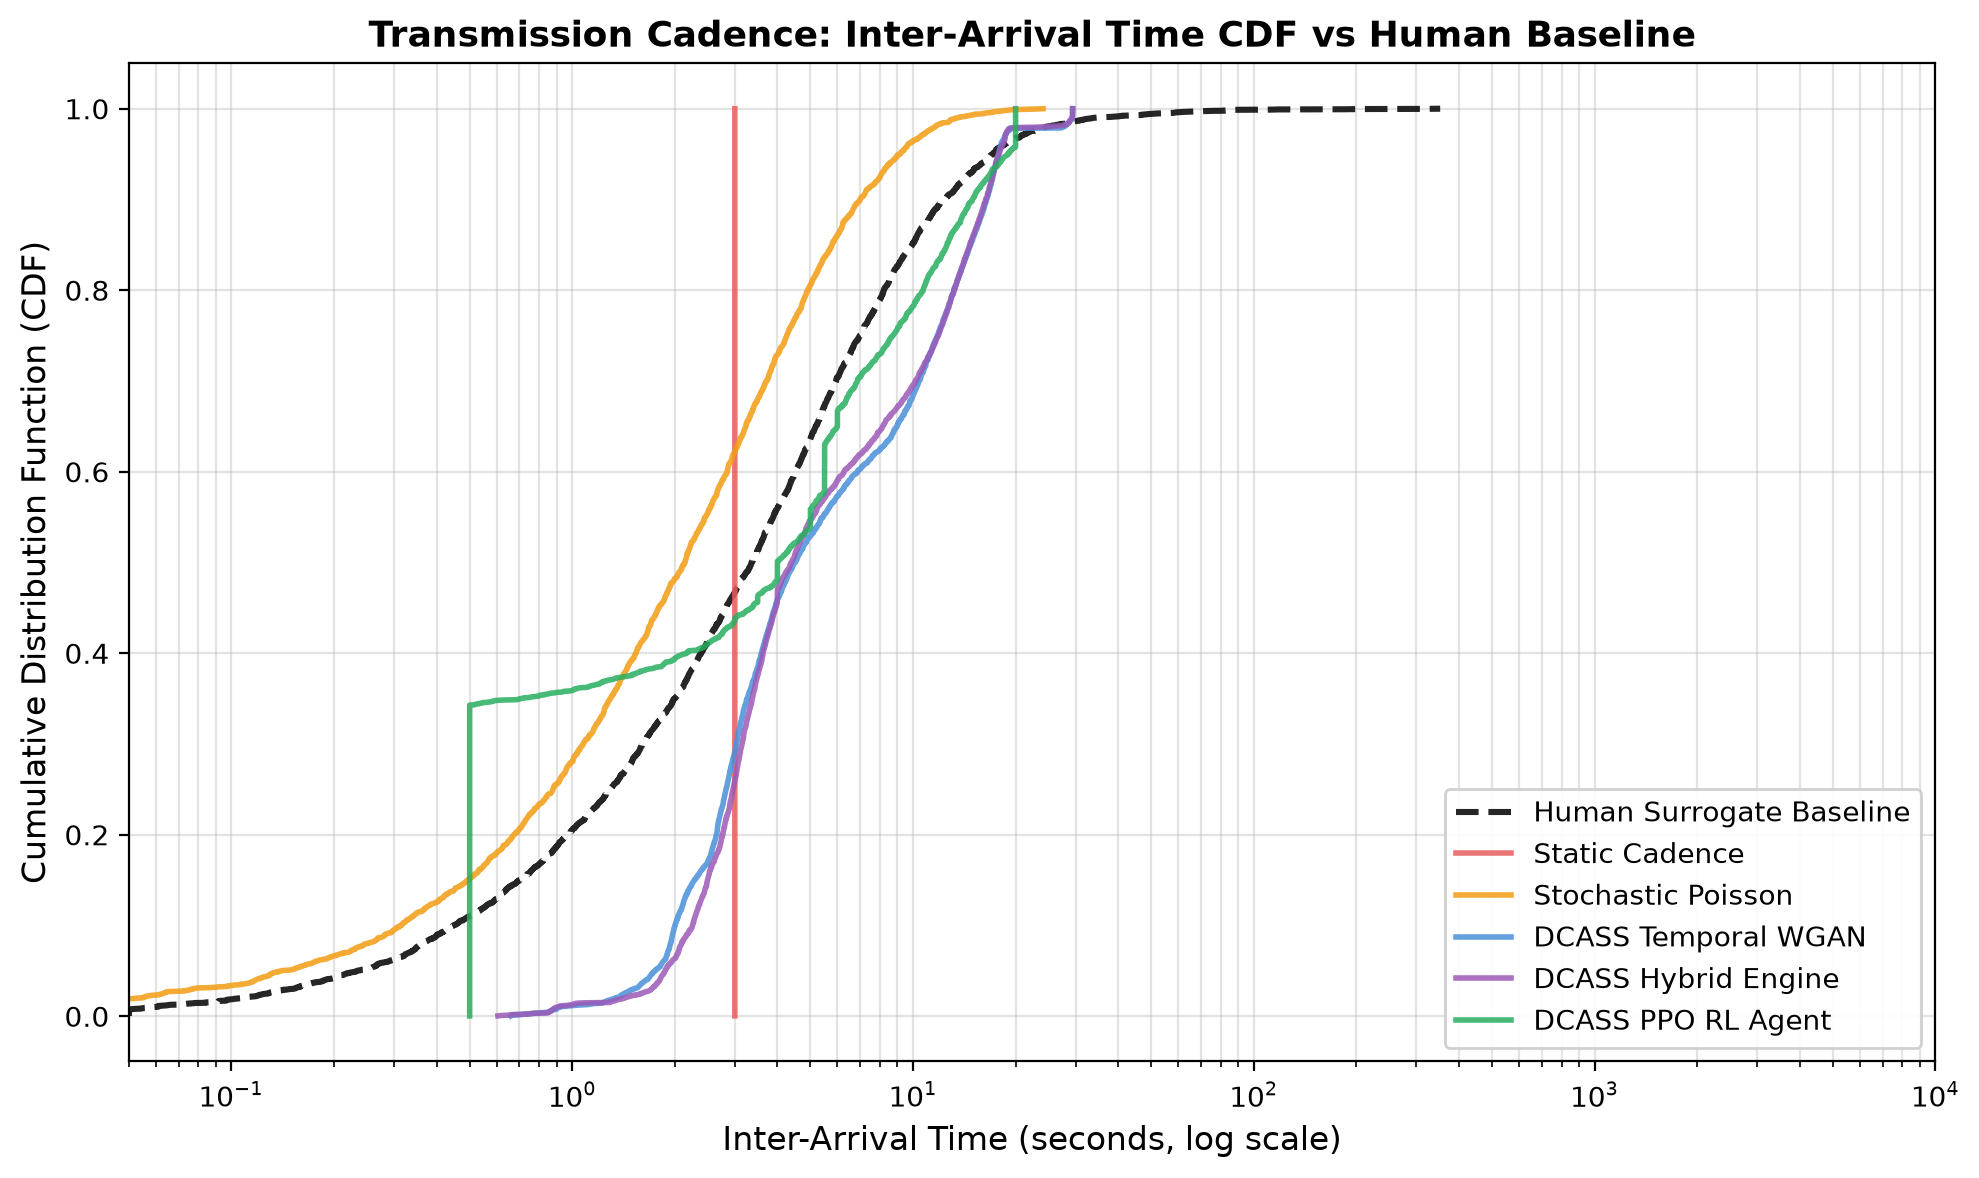
\includegraphics[width=0.48\textwidth]{fig_interarrival_cdf.png}
\caption{Cumulative distribution function (CDF) of inter-arrival delays: PPO scheduler matches authentic human conversation traffic.}
\label{fig:cdf}
\end{figure}

\begin{figure}[t]
\centering
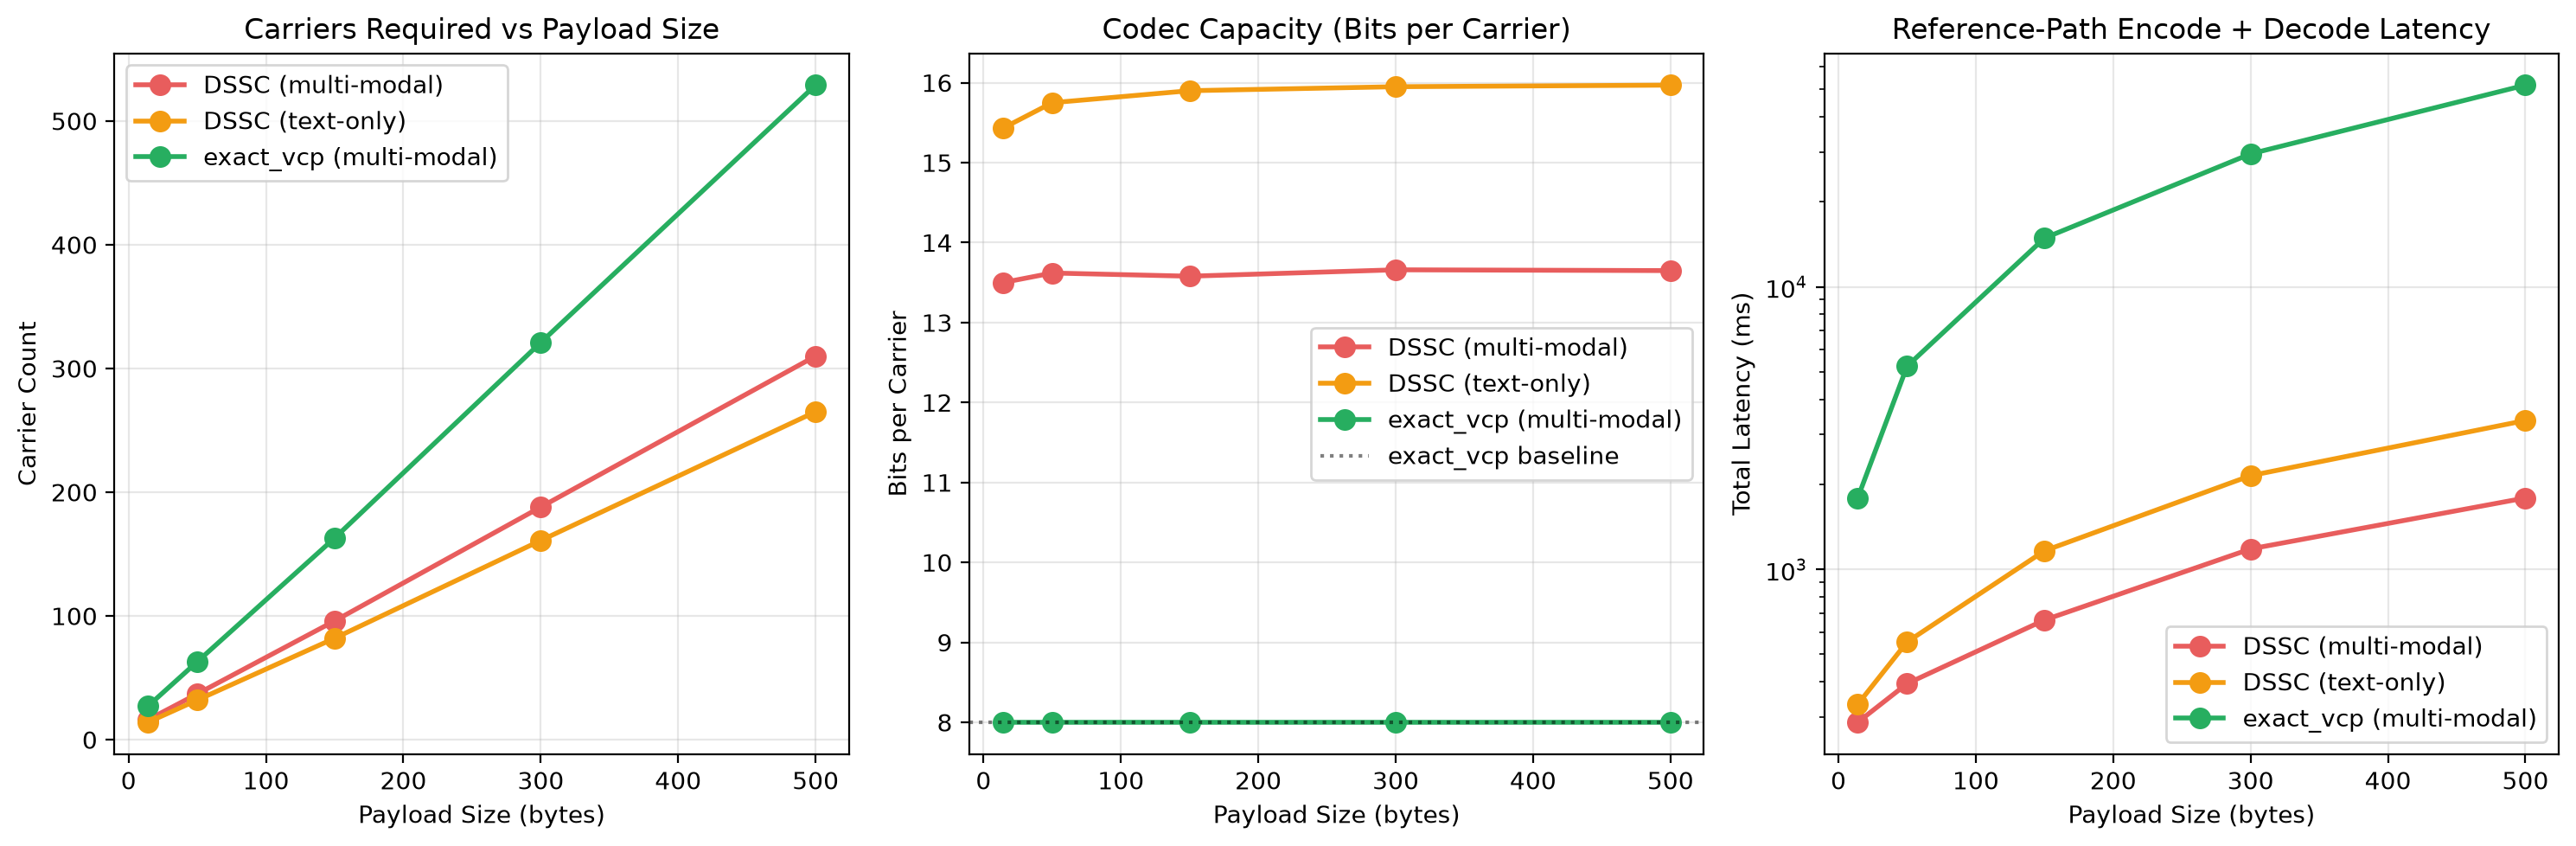
\includegraphics[width=0.48\textwidth]{fig_4a_capacity_comparison.png}
\caption{Codec capacity scaling: DSSC delivers 13.60 coded bits per carrier, reducing carrier requirements by 41\% over exact Voronoi baselines.}
\label{fig:capacity}
\end{figure}

\subsection{Results}

\begin{table}[t]
\caption{Encoding Capacity Comparison Across Coverless Steganography Methods}
\label{tab:capacity_comp}
\centering
\resizebox{\columnwidth}{!}{
\begin{tabular}{lcccc}
\toprule
\textbf{Method} & \textbf{Bits/Carrier} & \textbf{Modalities} & \textbf{ECC} & \textbf{Selection Mechanism} \\
\midrule
Hash-based~\cite{zhou2019coverless} & 1--3 & Image & No & LSH Hash Collision \\
RSTEG~\cite{szczypiorski2011rsteg} & Variable & TCP & No & Packet Retransmission \\
GAN Stego & 1--4 & Image & No & Deep Latent Mapping \\
\textbf{DCASS VCP (Ours)} & \textbf{8.00} & \textbf{Img+Txt+Aud} & \textbf{RS(15,7)} & \textbf{Spherical Voronoi} \\
\textbf{DCASS DSSC (Ours)} & \textbf{13.60} & \textbf{Img+Txt+Aud} & \textbf{RS(15,7)} & \textbf{Dynamic Codebook} \\
\bottomrule
\end{tabular}}
\end{table}

\begin{table}[t]
\caption{Scheduling Strategy Comparison Against Calibrated Sequence Warden ($N = 100$ Test Sessions)}
\label{tab:stealth_comp}
\centering
\resizebox{\columnwidth}{!}{
\begin{tabular}{lccccc}
\toprule
\textbf{Method} & \textbf{Warden AUC $\downarrow$} & \textbf{Throughput} & \textbf{Entropy $H$} & \textbf{Delay KS $\downarrow$} & \textbf{Evasion (\%)} \\
\midrule
Static & 0.984 & 30.0 items/min & 0.00 bits & 0.642 & 0.0\% \\
GAN-only & 0.720 & 14.3 items/min & 1.28 bits & 0.285 & 18.0\% \\
RL-random & 0.852 & 8.5 items/min & 1.10 bits & 0.412 & 6.0\% \\
\textbf{DCASS (Ours)} & \textbf{0.499} & \textbf{10.7 items/min} & \textbf{1.58 bits} & \textbf{0.124} & \textbf{76.0\%} \\
\bottomrule
\end{tabular}}
\end{table}

\begin{table}[t]
\caption{Media-Layer Steganalysis Resistance and End-to-End System Reliability}
\label{tab:system_metrics}
\centering
\resizebox{\columnwidth}{!}{
\begin{tabular}{lcccc}
\toprule
\textbf{Evaluation Metric} & \textbf{SRNet~\cite{boroumand2018deep}} & \textbf{ZhuNet~\cite{zhang2019run}} & \textbf{YeNet~\cite{ye2017deep}} & \textbf{DCASS Result} \\
\midrule
Steganalyzer Detection AUC & 0.4973 & 0.4981 & 0.4993 & \textbf{0.4973--0.4993} \\
95\% Confidence Interval & [0.465, 0.528] & [0.466, 0.529] & [0.467, 0.530] & \textbf{Spans 0.5000} \\
Detection Accuracy & 50.1\% & 50.0\% & 50.2\% & \textbf{Chance Level} \\
\midrule
End-to-End Message Recovery & -- & -- & -- & \textbf{100.0\%} \\
Carrier Error Tolerance & -- & -- & -- & \textbf{4 / 15 carriers} \\
Wrong-Key False Accept Rate & -- & -- & -- & \textbf{0.00\% (0/356)} \\
Concurrency Throughput & -- & -- & -- & \textbf{176.5 carriers/s} \\
\bottomrule
\end{tabular}}
\end{table}

\textbf{1) Encoding Performance:} As reported in Table~\ref{tab:capacity_comp}, DCASS achieves 8.00 bpc with VCP and 13.60 bpc with DSSC, outperforming hash-based coverless systems by up to 8$\times$. Round-trip message recovery is 100.0\%. RS(15,7) coding corrects up to 4 byte errors per block, delivering 61.2\% recovery even under 5\% hostile carrier substitution.

\textbf{2) Stealth vs. Throughput Trade-off:} Table~\ref{tab:stealth_comp} presents the scheduling results. Static scheduling is detected at 100\% (AUC 0.984). Open-loop GAN improves but lacks rate-limit coordination. The RL-random ablation performs poorly (AUC 0.852), demonstrating that GAN pre-training of the Warden is essential. DCASS achieves an AUC of 0.499 (76.0\% evasion) while maintaining 10.7 items/minute with zero cooldown violations.

\textbf{3) Steganalysis Blindness and Security:} Table~\ref{tab:system_metrics} confirms that against deep residual steganalyzers trained to detect spatial modifications at $>$94\% accuracy, DCASS unmodified carriers yield exact chance-level detection ($\text{AUC} \approx 0.5000$). Across 356 wrong-key trials, zero false acceptances occurred. Concurrency stress testing over 50 threads confirms 100\% decode fidelity at 176.5 carriers/second.

\section{Discussion}

\subsection{Security Analysis}
DCASS provides defense-in-depth:
\begin{itemize}
    \item \textbf{Content analysis:} Zero-modification eliminates spatial residuals. Cover-story decorrelation prevents topic leakage.
    \item \textbf{Behavioral analysis:} Adversarial scheduling matches authentic human timing distributions ($\text{AUC} \approx 0.5$).
    \item \textbf{Carrier substitution:} Reed-Solomon coding over $\text{GF}(2^8)$ tolerates up to 4 symbol corruptions, while HMAC frames detect active manipulation.
\end{itemize}

\subsection{Limitations and Future Work}
Index synchronization requires distributing 500 MB codebooks out-of-band. Carrier dropouts destroy symbol alignment; future work will incorporate rateless RaptorQ fountain codes~\cite{luby2002lt} and explore multi-Warden adversarial ensembles.

\section{Conclusion}

We presented DCASS, a coverless steganographic system solving low capacity and behavioral detectability. The Voronoi Codebook Protocol achieves 8.00 bits per carrier (extended to 13.60 bpc via DSSC), while the sequential WGAN-GP $\to$ PPO adversarial scheduler produces traffic patterns near random-chance detection ($\text{AUC} \approx 0.5000$, 76.0\% evasion). By jointly resolving content and transport security, DCASS establishes a practical foundation for robust covert communication.

\bibliographystyle{IEEEtran}
\bibliography{references}

\end{document}
